\documentclass[tikz,border=7pt]{standalone}
\usepackage{amsmath}
\usepackage{pgfplots}
\usepgfplotslibrary{groupplots}
\pgfplotsset{compat=1.18}
\definecolor{ink}{HTML}{17324D}
\definecolor{accent}{HTML}{0F766E}
\definecolor{gold}{HTML}{C28524}
\begin{document}
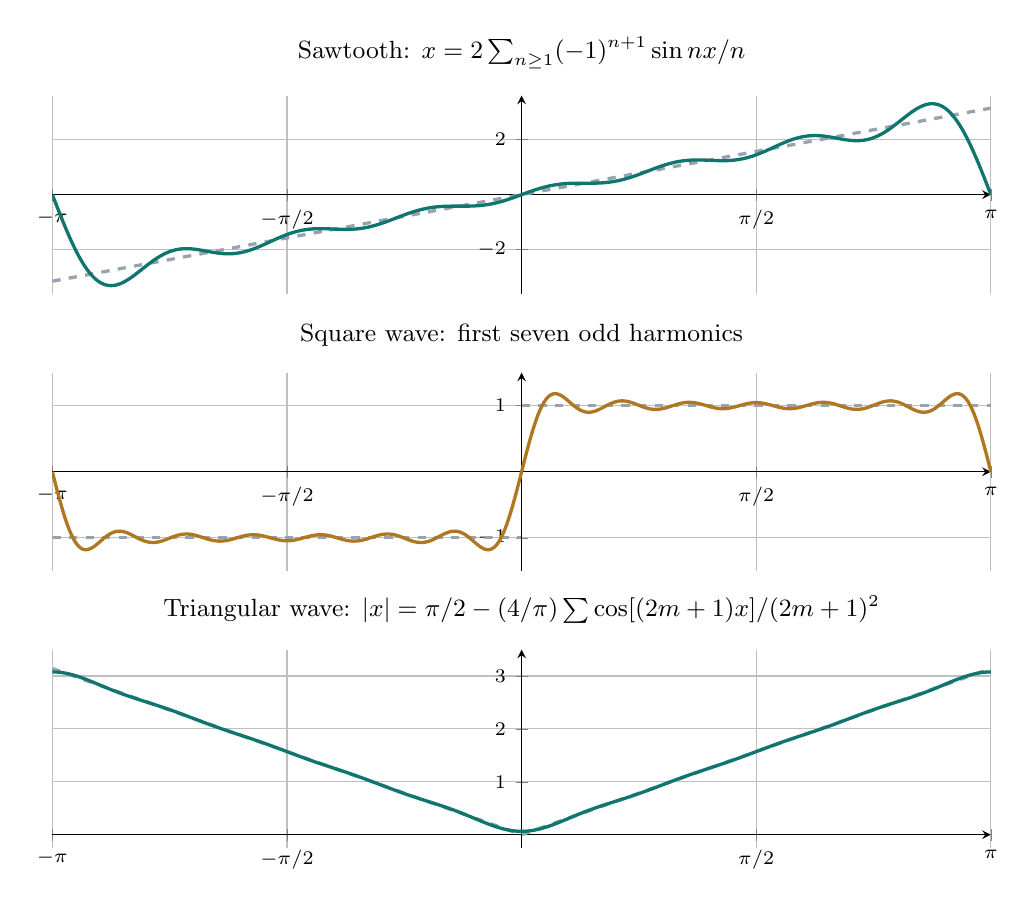
\begin{tikzpicture}
\begin{groupplot}[
 group style={group size=1 by 3,vertical sep=1.0cm},
 width=13.5cm,height=4.1cm,
 xmin=-3.1416,xmax=3.1416,
 axis lines=middle,grid=both,
 xtick={-3.1416,-1.5708,0,1.5708,3.1416},
 xticklabels={$-\pi$,$-\pi/2$,$0$,$\pi/2$,$\pi$},
 tick label style={font=\scriptsize},
 title style={font=\small},
]
\nextgroupplot[title={Sawtooth: $x=2\sum_{n\ge1}(-1)^{n+1}\sin nx/n$},ymin=-3.6,ymax=3.6]
 \addplot[ink!45,dashed,line width=1.2pt,domain=-3.1415:3.1415,samples=2]{x};
 \addplot[accent,very thick,domain=-3.1415:3.1415,samples=401]
 {2*(sin(deg(x))-sin(deg(2*x))/2+sin(deg(3*x))/3-sin(deg(4*x))/4+sin(deg(5*x))/5-sin(deg(6*x))/6+sin(deg(7*x))/7)};
\nextgroupplot[title={Square wave: first seven odd harmonics},ymin=-1.5,ymax=1.5]
 \addplot[ink!45,dashed,line width=1.2pt,domain=-3.1415:-.001,samples=2]{-1};
 \addplot[ink!45,dashed,line width=1.2pt,domain=.001:3.1415,samples=2]{1};
 \addplot[gold!90!black,very thick,domain=-3.1415:3.1415,samples=501]
 {(4/pi)*(sin(deg(x))+sin(deg(3*x))/3+sin(deg(5*x))/5+sin(deg(7*x))/7+sin(deg(9*x))/9+sin(deg(11*x))/11+sin(deg(13*x))/13)};
\nextgroupplot[title={Triangular wave: $|x|=\pi/2-(4/\pi)\sum\cos[(2m+1)x]/(2m+1)^2$},ymin=-.25,ymax=3.5]
 \addplot[ink!45,dashed,line width=1.2pt,domain=-3.1415:3.1415,samples=3]{abs(x)};
 \addplot[accent,very thick,domain=-3.1415:3.1415,samples=401]
 {pi/2-(4/pi)*(cos(deg(x))+cos(deg(3*x))/9+cos(deg(5*x))/25+cos(deg(7*x))/49+cos(deg(9*x))/81)};
\end{groupplot}
\end{tikzpicture}
\end{document}
